\documentclass[aspectratio=169]{beamer}
\usetheme{Madrid}
\usecolortheme{seahorse}
\setbeamertemplate{navigation symbols}{}
\setbeamertemplate{caption}[numbered]
\setbeamertemplate{itemize item}{\raise0.2ex\hbox{\tiny$\blacktriangleright$}}
\setbeamertemplate{itemize subitem}{\raise0.2ex\hbox{\tiny$\bullet$}}
\definecolor{hireblue}{HTML}{0F4C81}
\definecolor{hireteal}{HTML}{0E7490}
\setbeamercolor{structure}{fg=hireblue}
\setbeamercolor{frametitle}{fg=white,bg=hireblue}
\setbeamercolor{title}{fg=white,bg=hireblue}
\setbeamercolor{block title}{fg=white,bg=hireteal}
\setbeamercolor{block body}{bg=hireteal!8}
\usepackage[english]{babel}
\usepackage[T1]{fontenc}
\usepackage[utf8]{inputenc}
\usepackage{lmodern}
\usepackage{hyperref}
\usepackage{booktabs}
\usepackage{graphicx}
\usepackage{tabularx}
\usepackage{xcolor}
\usepackage{ragged2e}

\graphicspath{{../diagrams/}}

\hypersetup{
  colorlinks=true,
  linkcolor=blue,
  urlcolor=blue,
  pdftitle={Hire Lens Presentation}
}

\title[Hire Lens]{Hire Lens}
\subtitle{Cloud Computing Project Presentation}
\author{Mohammed Zaid Shaikh \and Piotr Bartosiewicz \and Krzysztof Krawiec}
\date{April 2026}

\begin{document}

\begin{frame}
  \titlepage
\end{frame}

\begin{frame}{Agenda}
  \tableofcontents
\end{frame}

\section{Project Overview}

\begin{frame}{The Problem}
\begin{columns}[T,onlytextwidth]
  \column{0.58\textwidth}
  \justifying
  Hire Lens helps HR teams screen candidates faster by turning public GitHub activity into a structured review and a job-match summary.

  \vspace{0.5em}
  The first release stays practical, explainable, and cheap to run while leaving room for AI-assisted ranking later.
  \column{0.38\textwidth}
  \begin{block}{Primary Users}
    \begin{itemize}
      \item Recruiters
      \item Team leads
      \item Platform admins
    \end{itemize}
  \end{block}
\end{columns}
\end{frame}

\begin{frame}{What Hire Lens Does}
\begin{enumerate}
  \item Accepts a GitHub username or profile link through Telegram.
  \item Collects public signals such as repositories, languages, activity, and followers.
  \item Produces a concise candidate summary and later a job-description comparison.
  \item Stores reports so recruiters can revisit and shortlist candidates.
  \item Enforces basic usage limits and prepares the path for paid tiers.
\end{enumerate}

\vspace{0.5em}
\begin{block}{Design Choice}
Telegram stays the main interface; a small dashboard is optional, not central.
\end{block}
\end{frame}

\section{Solution Design}

\begin{frame}{Architecture at a Glance}
\begin{columns}[T,onlytextwidth]
  \column{0.44\textwidth}
  \begin{itemize}
    \item Telegram bot as the frontend
    \item Azure Functions for API and webhook handling
    \item Azure Container Apps for the self-hosted model service
    \item Cosmos DB and Blob Storage for data
    \item Service Bus for asynchronous jobs
  \end{itemize}
  \column{0.54\textwidth}
  \centering
  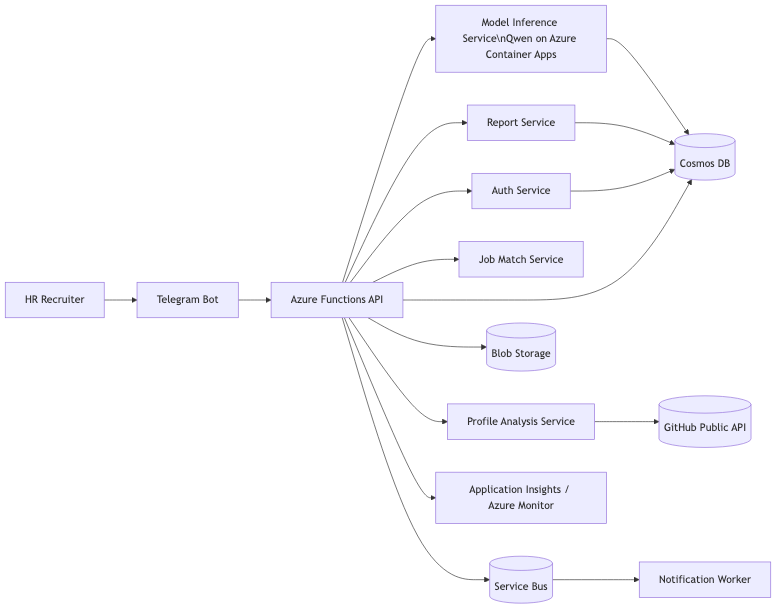
\includegraphics[width=\linewidth,height=0.62\textheight,keepaspectratio]{architecture.png}
\end{columns}
\end{frame}

\begin{frame}{Request Flow}
\begin{columns}[T,onlytextwidth]
  \column{0.36\textwidth}
  \begin{enumerate}
    \item Recruiter sends a GitHub profile.
    \item Bot triggers analysis through Azure Functions.
    \item Public data is enriched and summarized.
    \item Results are stored and returned in Telegram.
  \end{enumerate}
  \column{0.60\textwidth}
  \centering
  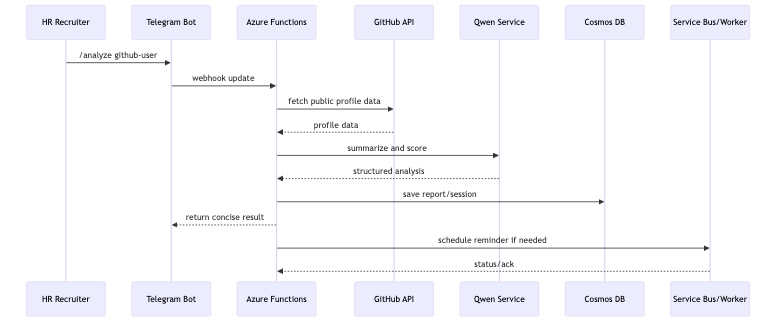
\includegraphics[width=\linewidth,height=0.62\textheight,keepaspectratio]{request-flow.png}
\end{columns}
\end{frame}

\begin{frame}{Storage and Infrastructure}
\begin{columns}[T,onlytextwidth]
  \column{0.52\textwidth}
  \begin{block}{Storage}
    \begin{itemize}
      \item Cosmos DB for users, sessions, reports, and limits
      \item Blob Storage for exports and cached snapshots
      \item Optional SQL/Table storage for audit and billing records
    \end{itemize}
  \end{block}
  \begin{block}{Terraform}
    \begin{itemize}
      \item Separate modules for functions, data, messaging, and monitoring
      \item Dev first, then prod
    \end{itemize}
  \end{block}
  \column{0.42\textwidth}
  \centering
  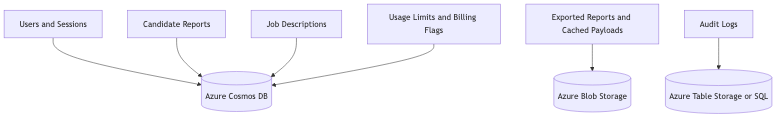
\includegraphics[width=\linewidth,height=0.62\textheight,keepaspectratio]{storage.png}
\end{columns}
\end{frame}

\section{Delivery}

\begin{frame}{Risks and Mitigations}
\begin{itemize}
  \item GitHub API limits: reduce calls with caching and queueing.
  \item AI quality: keep a deterministic fallback summary path.
  \item Hosting cost: start with a smaller quantized model and strict rate limits.
  \item OAuth complexity: begin with one provider, then expand.
  \item External costs: prefer the cheapest practical Azure region and usage caps.
\end{itemize}
\end{frame}

\begin{frame}{Team Split and Milestones}
\begin{columns}[T,onlytextwidth]
  \column{0.48\textwidth}
  \begin{block}{Responsibilities}
    \begin{itemize}
      \item Mohammed Zaid Shaikh: bot flow and UX
      \item Piotr Bartosiewicz: analysis logic and APIs
      \item Krzysztof Krawiec: Terraform, deployment, monitoring
    \end{itemize}
  \end{block}
  \column{0.44\textwidth}
  \begin{block}{Milestones}
    \begin{enumerate}
      \item Telegram login and profile analysis
      \item Report storage and retrieval
      \item Job matching and usage limits
      \item Terraform deployment and demo
    \end{enumerate}
  \end{block}
\end{columns}
\end{frame}

\begin{frame}{Closing}
Hire Lens is intentionally small in the first release: one bot, one backend, managed Azure services, and a clear path to AI-assisted hiring support.
\end{frame}

\end{document}